
\textbf{System Architecture.}
As shown in Fig.~\ref{fig:hivewatch}, HiveWatch is designed as a
framework-agnostic observability layer for federated and distributed machine
learning workloads. The federated learning framework remains responsible for
client selection, model distribution, local training, and aggregation. HiveWatch
is inserted at the server-side control flow, where it records round starts,
client updates, aggregate round summaries, failures, and experiment metadata.
This design allows HiveWatch to support APPFL, Flower, NVFlare, and custom
training loops without requiring changes to the underlying communication
protocol or aggregation algorithm.

\begin{figure*}[t]
    \centering
    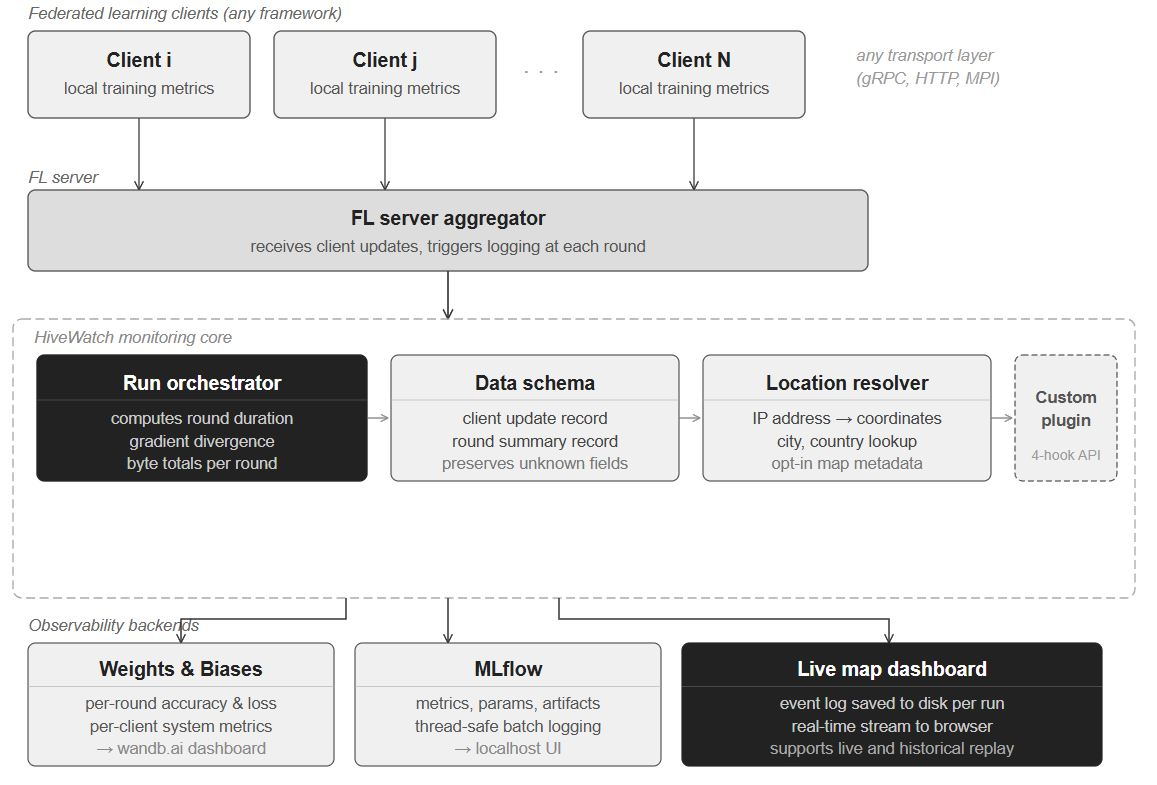
\includegraphics[width=0.9\linewidth]{images/arch.JPG}
    \caption{Overview of the HiveWatch monitoring framework.}
    \label{fig:hivewatch}
\end{figure*}

% \begin{figure}[t]
%     \centering
%     % If using the svg package:
%     \includesvg[width=\columnwidth]{images/hivewatch_architecture.svg}
%     % If converted to PDF instead, use:
%     % \includegraphics[width=\columnwidth]{hivewatch_architecture.pdf}
%     \caption{Architecture of HiveWatch. Federated clients train on local data
%     and return model updates with metadata. The FL server invokes the HiveWatch
%     runtime API, which normalizes events and forwards them to local replay
%     artifacts, a map dashboard, MLflow, and Weights \& Biases.}
%     \label{fig:hivewatch-architecture}
% \end{figure}
\textbf{Runtime Instrumentation.}
HiveWatch exposes a small runtime API consisting of three primary calls:
\texttt{round\_start()}, \texttt{log\_client\_update()}, and
\texttt{log\_round()}. During each training round, the server marks the start
of the round, records each client update as it arrives, and logs the final
round-level summary after aggregation. Client updates may include local
accuracy, local loss, number of samples, gradient statistics, communication
volume, training time, system utilization, geographic metadata, and client
status. Unknown framework-specific fields are preserved, allowing applications
to attach custom metadata without modifying HiveWatch's core schema.

\textbf{Emitter Backends.}
HiveWatch decouples metric collection from metric storage through a pluggable
emitter interface. The same event stream can be sent to multiple destinations.
The SSE emitter writes replayable JSONL event logs and map-ready metadata
artifacts, enabling local inspection and deferred analysis. The MLflow emitter
records metrics, parameters, tags, and artifacts for self-hosted experiment
tracking. The Weights \& Biases emitter supports hosted dashboards, per-client
metrics, and alert-style events for failures or dropouts. This emitter-based
design lets users choose local, hosted, or hybrid monitoring workflows.

\textbf{Replay and Map Visualization.}
In addition to scalar experiment tracking, HiveWatch provides a local dashboard
for visualizing geographically distributed clients. The dashboard consumes
saved \texttt{.jsonl} and \texttt{.map.json} artifacts, allowing users to
inspect both live runs and completed runs. Client locations, training status,
round progress, failures, and non-geographic metadata are displayed in a
single replayable view. This is useful for diagnosing stragglers, communication
failures, anomalous clients, and non-IID behavior in distributed experiments.